\title{Q-compensated denoising of seismic data}
\renewcommand{\thefootnote}{\fnsymbol{footnote}}
\author{Hang Wang, Guangtan Huang, Yangkang Chen, and Wei Chen}
%\thanks{H. Wang, G. Huang, Y. Chen are with Zhejiang University.}
%\thanks{W. Chen is with Yangtze University (corresponding author).}
%\thanks{The research is supported by the National Natural Science Foundation of China (Grant No. 41804140).}}
\maketitle




\begin{abstract}
It is widely known that strong noise can decrease the quality of seismic data. However, the anelastic attenuation could be more important to account for the weak amplitude and low quality of seismic data. Here, we develop an inversion framework to simultaneously compensate for the attenuation of seismic data and remove noise, thereby enhancing the quality of seismic data. Instead of directly applying a compensation operator to the input seismic data, we formulate an inverse problem that connects the sparse reflectivity model and the raw seismic data % that is attenuated and noisy 
via the convolution and attenuation functions. The random noise is assumed to be the unpredicted part \old{in}\new{of} the forward modeling process. We use the L2-norm regularization for the data misfit and impose a sparsity constraint onto the reflectivity series, e.g., using the L1-norm constraint. We use an iterative preconditioned conjugate gradient method to solve the L1-norm constrained least-squares optimization problem and obtain the  reflectivity series. The denoised and compensated data is obtained by applying the convolution operator to the reflectivity. We use several synthetic and field seismic data to illustrate the effectiveness of the presented method.
\end{abstract}

%\begin{keywords}
%Q-compensation, denoising, and seismic data
%\end{keywords}

\section{Introduction}
Recovering the seismic signals from the strong background seismic noise, also known as seismic denoising, is of great importance of the whole seismic data processing chain \cite[]{yanan2014,yanhui2016,amir2017ieee,li2018multidimensional,wang2019hankel}.  There have been a lot of classic denoising algorithms in the literature, e.g., the prediction-based denoising methods \cite[]{canales1984,abma1995}, \new{the sparse transform based denoising methods \cite[]{fomel2010seislet,mostafa2016geo,mostafa2016bssa,mousavi2017automatic}}, the mode decomposition based denoising methods \cite[]{chenwei2012}, the rank-reduction based denoising methods \cite[]{mssa,weilin2016dmssa,zhaoqiang2019tgrs}, etc. Despite \old{of }the reported success in the field of seismic denoising, the traditional methods cannot resolve the problem of amplitude loss due to the anelastic attenuation when seismic waves are propagated in subsurface media. \new{The amplitude loss could make the recorded seismic data contain very weak events.} This limitation makes all traditional seismic denoising methods fail in dealing with highly attenuated seismic data, e.g., the weak seismic signals. What is worse is that due to the weak energy of those attenuated seismic events, the spatial correlation is also mitigated, thereby causing a high probability in damaging the weak events during the denoising process. \new{Besides, most denoising methods also affect the amplitude, thus causing a high chance that the attenuation estimation using denoised signal results in overestimation of the quality factor, Q.} In this paper, we will focus on the challenging problem of simultaneous denoising and attenuation compensation (Q-compensation). The goal is to develop an inversion framework that \old{can }not only \new{can} attenuate the random noise, but also compensate for the anelastic amplitude loss and thus increase the vertical resolution.  

The anelastic attenuation is usually described by the quality factor (Q). Kjartansson (1979) \cite[]{kjartansson1979constant} proposed a constant Q-model, which describes an attenuation medium \cite[]{bickel1985plane,wang2002stable,shen2018q,shen2018q2}. In the constant Q-model, the quality factor does not vary with frequency \cite[]{braginsky1989quality,dai2012multi}. The estimation of Q is important in a variety of geophysical inverse problems, e.g., Q-compensated seismic migration, high-fidelity seismic interpretation, reservoir fluid characterization, and seismic risk estimation \cite[]{mousavi2014jgr,shank2018image,cheng2018q,jyothi2017seismic,luo2019q,chen2019multichannel}. Q-compensation, a widely used method to seismic imaging, is becoming a \old{heated}\new{hot} researching topic in exploration geophysics \cite[]{guo2017adjoint,zhou2019viscoacoustic,aharchaou2019prestack}. \new{Besides, Q can also be used to interpret the large-scale geological features \cite[]{zhao2018lateral}.}

Reverse time migration (RTM) is thought as one of the most effective seismic imaging methods \cite[]{baysal1983reverse,yoon2004challenges,dai2012multi}. In recent years, Q-compensation research for different forms of reverse time migration has emerged. \cite[]{zhang2010compensating} proposed a Q-compensated RTM, where a \old{viscoelastic}\new{viscoacoustic} wave equation is used for compensating amplitude attenuation and phase dispersion effects.  Researchers also used the separated fractional Laplace equation to approximate the constant-Q wave equation for viscous acoustic medium modeling and imaging tasks \cite[]{zhu2014q,fathalian2020approach}, which plays an important role in effectively using constant-Q in data processing \cite[]{harris2014q,wang2018adaptive}.\old{ The viscoelastic least-square inverse time migration (also known as Q-LSRTM) is a linear inversion of \new{a} subsurface reflectance model from lossy data ?. Compared with the traditional migration method, it could compensate for the amplitude loss of the migration image caused by the strong underground attenuation, and can produce the reflector accurately located at the depth. Researchers have developed different algorithms and demonstrate the Q-LSRTM method converges significantly faster than least-square reserve time migration ?.} Q-compensation can be utilized in full waveform inversion (FWI) as well. FWI provides a reliable method for the establishment of \new{a} high-resolution underground model, especially for the construction of \new{a} complex geological structure model, which has been \old{fully}\new{extensively} studied\old{ and developed} in the past decades \cite[]{tarantola2005inverse,virieux2009overview}. Q-compensated FWI has been proved to be highly effective \new{for building a reliable subsurface velocity model} \cite[]{xue2018accelerating}. \old{By comparing the convergence rates of FWI with Q-compensated gradient and without Q-compensated gradient, we can know that the Q-compensation strategy can obviously improve the convergence of FWI, which is helpful for the fast inversion of \new{the} deep structure of velocity model ?. \old{However, attenuation reconstruction is always an ill-posed problem. Because the reliability of attenuation reconstruction depends on the precision of \new{the} initial velocity model to a great extent, FWI has the advantages of being more robust and stable, but the calculation cost is very high ?.} ? proposed a ray based Q-tomography, which can be incorporated into the traditional depth velocity modeling process. In order to compensate for the attenuation in RTM and FWI imaging, it is necessary to estimate the spatial change rate of attenuation from the dataset. Q-tomography based on frequency shift data is very useful in estimating the uniform attenuation rate ?.}

%Q-compensation can be utilized in full waveform inversion (FWI) as well. FWI provides a reliable method for the establishment of \new{a} high-resolution underground model, especially for the construction of \new{a} complex geological structure model, which has been \old{fully}\new{extensively} studied\old{ and developed} in the past decades \cite[]{tarantola2005inverse,virieux2009overview}. Q-compensated FWI has been proved to be highly effective \new{for building a reliable subsurface velocity model} \cite[]{xue2017visco,xue2018accelerating}. By comparing the convergence rates of FWI with Q-compensated gradient and without Q-compensated gradient, we can know that the Q-compensation strategy can obviously improve the convergence of FWI, which is helpful for the fast inversion of \new{the} deep structure of velocity model \cite[]{alasmri2019towards,li2016application,xue2016q,wang2019q}. \old{However, attenuation reconstruction is always an ill-posed problem. Because the reliability of attenuation reconstruction depends on the precision of \new{the} initial velocity model to a great extent, FWI has the advantages of being more robust and stable, but the calculation cost is very high ?.} \cite[]{xin20093} proposed a ray based Q-tomography, which can be incorporated into the traditional depth velocity modeling process. In order to compensate for the attenuation in RTM and FWI imaging, it is necessary to estimate the spatial change rate of attenuation from the dataset. Q-tomography based on frequency shift data is very useful in estimating the uniform attenuation rate \cite[]{harris2014q,he2012q,xin2014robust}.
	
\old{Furthermore, Q-compensation is useful for non-linear reconstruction of seismic reflection data, which has been proved for its the concept and numerical feasibility, and also with more robustness ?. What is more, Q-compensation technology could contribute to tomography for complex near-surface condition. Since the Q-compensation strategy can significantly boost the energy that is lost due to the attenuation of the high-frequency components in the shallow to middle layers ?.} \new{While the Q-compensation problem has been extensively studied in either an independent processing step or in the wave-equation based imaging step via RTM and FWI, it is seldom investigated in conjuction with the seismic denoising process. As we know, seismic attenuation affects the seismic denoising since it could extra-weak seismic reflections while denoising also affects Q compensation greatly because denoising could weaken the seismic signals that are closely related with the Q estimation. Here, we propose an integrated framework for simultaneously denoising and Q compensation. } In this paper, we will start from the basic convolution model and then introduce the forward operator in the frequency domain that incorporates the anelastic attenuation. We will introduce a preconditioned conjugate gradient method to solve for the Q-compensated reflectivity inversion, after which we can obtain the Q-compensated amplitude recovery with the random noise simultaneously removed.

\subsection{Convolution model with anelastic attenuation}
The convolution model is well known as:
\begin{equation}
\label{eq:conv}
\mathbf{d} = \mathbf{Wr},
\end{equation}
where $\mathbf{d}$ denotes the seismic data, $\mathbf{W}$ denotes the convolution matrix that is composed of the source wavelet $\mathbf{w}$, and $\mathbf{r}$ denotes the reflectivity. When considering the subsurface seismic anelastic attenuation, the convolution model \ref{eq:conv} can be modified as:
\begin{equation}
\label{eq:conva}
\mathbf{d} = \mathbf{WAr},
\end{equation}
where $\mathbf{A}$ denotes the attenuation operator. In an integral form, equation \ref{eq:conva} can be expressed as \cite[]{margrave2011gabor,yufeng2018l12}:
\begin{equation}
\label{eq:int}
d(\omega) = w(\omega) \int r(t)a(\omega,t)e^{-i\omega t}dt,
\end{equation}
where $d(\omega)$ and $w(\omega)$ denote the spectrum of the seismic data $d(t)$ and wavelet function $w(t)$ in the frequency domain, respectively. $a(\omega,t)$ corresponds to an attenuation function. $r(t)$ is the reflectivity function in the time domain. The attenuation function can be defined based on the constant-Q theory as follows \cite[]{zhu2014q,yufeng2018l12}:
\begin{equation}
\label{eq:af}
a(\omega, t) = e^{-\frac{\omega t}{2Q}\left | \frac{\omega}{\omega_h} \right |^{-\gamma}}e^{i \omega t \left | \frac{\omega}{\omega_h} \right |^{-\gamma}},
\end{equation}
where $\gamma=\frac{1}{\pi Q}$, and $\omega_h$ is a reference frequency \new{e.g., 30 Hz}. 

According to equation \ref{eq:int}, the explicit expression of equation \ref{eq:conva} can be written as:
\begin{equation}
\label{eq:exp}
\begin{split}
&\left[ \begin{array}{ccc}
e^{-i \omega_1 t_1}w(\omega_1)a(\omega_1, t_1) & \ldots & e^{-i \omega_1 t_N}w(\omega_1)a(\omega_1, t_N) \\
\vdots & \ddots & \vdots \\
e^{-i \omega_M t_1}w(\omega_M)a(\omega_M, t_1) & \ldots & e^{-i \omega_M t_N}w(\omega_M)a(\omega_M, t_N)
\end{array} \right] \\
&\left[\begin{array}{c} r_1 \\ \vdots \\ r_N \end{array} \right] = \left[\begin{array}{c} d(\omega_1) \\ \vdots \\ d(\omega_M) \end{array} \right] .
\end{split}
\end{equation}

\begin{figure}[htb!]
 \centering
 \subfloat[]{\includegraphics[width=0.22\textwidth]{synth/Fig/syn-dc}
   \label{fig:syn-dc}}\\
 \subfloat[]{\includegraphics[width=0.22\textwidth]{synth/Fig/syn-da}
   \label{fig:syn-da}}
 \subfloat[]{\includegraphics[width=0.22\textwidth]{synth/Fig/syn-dn}
   \label{fig:syn-dn}}
  \caption{Synthetic data example. \old{(a) Clean data. (b) Noisy data with attenuated amplitude. (c) Enhanced data using fx method. (d) Enhanced data using the proposed method.}\new{(a) Clean data. (b) Clean data with attenuated amplitude. (c) Noisy data with attenuated amplitude.}}
  \label{fig:syn-dc,syn-da,syn-dn}
\end{figure}

\begin{figure}[htb!]
 \centering
 \subfloat[]{\includegraphics[width=0.22\textwidth]{synth/Fig/syn-d2}
   \label{fig:syn-d2}}
 \subfloat[]{\includegraphics[width=0.22\textwidth]{synth/Fig/syn-d1}
   \label{fig:syn-d1}}
  \caption{Synthetic data example. (a) Denoised data using FX method. (d) Q-compensated and denoised data using the proposed method.}
  \label{fig:syn-d2,syn-d1}
\end{figure}


\begin{figure}[htb!]
 \centering
 \subfloat[]{\includegraphics[width=0.22\textwidth]{synth/Fig/syn-da-simi}
   \label{fig:syn-da-simi}}
 \subfloat[]{\includegraphics[width=0.22\textwidth]{synth/Fig/syn-dn-simi}
   \label{fig:syn-dn-simi}}\\
 \subfloat[]{\includegraphics[width=0.22\textwidth]{synth/Fig/syn-d2-simi}
   \label{fig:syn-d2-simi}}
 \subfloat[]{\includegraphics[width=0.22\textwidth]{synth/Fig/syn-d1-simi}
   \label{fig:syn-d1-simi}}
  \caption{Similarity comparison between the target data and the ground truth for (a) attenuated data, (b) noisy data, (c) denoised data using FX method, and (d) the proposed method.}
  \label{fig:syn-da-simi,syn-dn-simi,syn-d2-simi,syn-d1-simi}
\end{figure}


\begin{figure}[htb!]
 \centering
 \subfloat[]{\includegraphics[width=0.5\textwidth]{synth/Fig/syn-ss0}
   \label{fig:syn-ss0}}
 \subfloat[]{\includegraphics[width=0.5\textwidth]{synth/Fig/syn-ss-z}
   \label{fig:syn-ss-z}}
  \caption{Trace-by-trace (3rd trace in Figs. \ref{fig:syn-dc,syn-da,syn-dn} and \ref{fig:syn-d2,syn-d1}) comparison for the synthetic data example, in the original scale (a), and in the zoomed scale (b). The red line denotes the clean attenuated data. The pink line corresponds to the noisy attenuated data. The green line corresponds to the Q-compensated denoising method. The blue line corresponds to the FX method.  The black line corresponds to the ground truth. It is clear that the black and green lines are close to each other.}
  \label{fig:syn-ss0,syn-ss-z}
\end{figure}

\begin{figure}[htb!]
 \centering
 \subfloat[]{\includegraphics[width=0.23\textwidth]{field/Fig/real-dn-0}
   \label{fig:real-dn-0}}\\
 \subfloat[]{\includegraphics[width=0.23\textwidth]{field/Fig/real-d2-0}
   \label{fig:real-d2-0}}
 \subfloat[]{\includegraphics[width=0.23\textwidth]{field/Fig/real-d1-0}
   \label{fig:real-d1-0}}   
  \caption{Field data example. (a) Raw data. (b) Enhanced data using fx method. (c) Enhanced data using the proposed method.}
  \label{fig:real-dn-0,real-d2-0,real-d1-0}
\end{figure}

\subsection{Q-compensated seismic denoising}
%The nonstationary convolution in the frequency domain, we can solve the following optimization problem for the sparse reflectivity. 
Let $\mathbf{F}=\mathbf{WA}$, then equations \ref{eq:conva} and \ref{eq:exp} can be briefly expressed as
\begin{equation}
\label{eq:inv}
\mathbf{d} = \mathbf{Fr},
\end{equation}
which can be solved via the regularized optimization method
\begin{equation}
\label{eq:cost1}
\hat{\mathbf{r}} = \arg \min_{\mathbf{r}} \ \frac{1}{2} \parallel \mathbf{F} \mathbf{r}-\mathbf{d}\parallel_2^2+ \lambda \parallel\mathbf{r}\parallel_1,
\end{equation}
where $\parallel\cdot \parallel_2$ denotes the $L_2$-norm data misfit and $\parallel\cdot \parallel_1$ denotes the $L_1$-norm model constraint. $\lambda$ denotes a the compromising parameter that controls the weight between the data misfit and model constraint. 

Note that 
\begin{equation}
\label{eq:l1l2}
\parallel \mathbf{r} \parallel_1 = \sum_{i} |r_i| =  \sum_{i} |r_i| |r_i|^{-1} |r_i| = \parallel \mathbf{W}_r\mathbf{r} \parallel_2^2,
\end{equation}
where $[\mathbf{W}_r]_{ii}=|r_i|^{-1/2}$. To avoid the singularity caused by too small $r_i$, a threshold needs to be defined \cite[]{amr2014}. 

Substituting equation \ref{eq:l1l2} into equation \ref{eq:cost1}, we obtain
\begin{equation}
\label{eq:cost2}
\hat{\mathbf{r}} = \arg \min_{\mathbf{r}} \ \frac{1}{2} \parallel \mathbf{F} \mathbf{r}-\mathbf{d}\parallel_2^2+ \lambda \parallel \mathbf{W}_r\mathbf{r} \parallel_2^2,
\end{equation}
which can then be transformed as
\begin{equation}
\label{eq:cost2}
\hat{\mathbf{m}} = \arg \min_{\mathbf{m}} \ \frac{1}{2} \parallel \mathbf{F} \mathbf{W}_r^{-1}\mathbf{m}-\mathbf{d}\parallel_2^2+ \lambda \parallel \mathbf{m} \parallel_2^2,
\end{equation}
by defining $\mathbf{r}=\mathbf{W}_r^{-1}\mathbf{m}$.

Equation \ref{eq:cost2} can be solved via the classic conjugate gradient method. In summary, when solving equation \ref{eq:cost1}, we need to iteratively solve for $\mathbf{m}$ and $\mathbf{W}_r$. $\mathbf{W}_r$ needs to be re-calculated during the iterations. \new{Following Daniel (2003) \cite[]{daniel2003}}, we ease the inconvenience in selecting the balancing parameter $\lambda$ by adjusting the sparsity constraint through the number of re-weighting iterations. A higher number of re-weighting iterations corresponds to a higher trade-off parameter $\lambda$ and vice versa. The detailed preconditioned conjugate gradient algorithm to solve equation \ref{eq:cost1} is provided in Algorithm \ref{alg:alg1}, where the input are the forward operator $\mathbf{F}$, raw data $\mathbf{d}$, and initial guess of $\mathbf{m}_0$, inner and outer iterations $N_i$ and $N_o$. When the  reflectivity $\hat{\mathbf{r}}=\mathbf{r}_{N_i}$ is solved through algorithm \ref{alg:alg1}, the Q-compensated and denoised data can be obtained by $\hat{\mathbf{s}} = \mathbf{W}\hat{\mathbf{r}}$.

\new{The proposed method is based on 1D assumption, which means that we need to apply the Q-compensation algorithm in post-stack data. Besides, in this paper, we do not seek a theoretically correct Q-compensation result. Instead, we seek an improved version of denoising, where the Q effect is taken into consideration. Also, we demonstrate that even thorough a roughly assumed constant Q value, we can obtain significant improvement of the SNR and resolution of the result, as detailed in the next section. }
\begin{algorithm}
   \caption{Iterative preconditioned conjugate gradient algorithm}
   \textbf{Input:} $\mathbf{d}$,$\mathbf{m}_0$,$N_o$,$N_i$,$\mathbf{F}$ \\
   \textbf{Output:} $\hat{\mathbf{r}}$ 
    \begin{algorithmic}[1]
    \State $\mathbf{W}_r=\mathbf{I}$
    \State $\mathbf{r}_0=\mathbf{W}_r\mathbf{m}_0$ 
    \For {$t = 1:N_o$}
    \State $\mathbf{r}_0=\mathbf{d}-\mathbf{F}\mathbf{W}_r\mathbf{m}_0$
    \State $\mathbf{W}_r=\text{diag}(\mathbf{r}_0^{1/2})$
    \State $\mathbf{p}_0=\mathbf{W}_r^T\mathbf{F}^T\mathbf{r}_0$;$\quad$$\mathbf{p}_1=\mathbf{p}_0$ 
    \State $\mathbf{u}_0=\mathbf{p}_0$;$\quad$$\mathbf{u}_1=\mathbf{u}_0$ 
    \For {$k = 1:N_i$}
    \State $\mathbf{q}_{N_i}=\mathbf{F}\mathbf{W}_r\mathbf{u}_{N_i}$
    \State $\alpha=\mathbf{p}_{N_i}^T\mathbf{p}_{N_i}/\mathbf{q}_{N_i}^T\mathbf{q}_{N_i}$
    \State $\mathbf{m}_{N_i}=\mathbf{m}_{k-1}+\alpha\mathbf{p}_{N_i}$
    \State $\mathbf{r}_{N_i}=\mathbf{r}_{k-1}-\alpha\mathbf{q}_{N_i}$ 
    \State $\mathbf{p}_{N_i}=\mathbf{W}_r^T\mathbf{F}^T\mathbf{r}_{N_i}$
    \State $\beta=\mathbf{r}^T_{k}\mathbf{r}_{k}/\mathbf{r}^T_{k-1}\mathbf{r}_{k-1}$ 
    \State $\mathbf{u}_{N_i}=\mathbf{p}_{N_i}+\beta\mathbf{u}_{N_i}$
%    \If {$\textbf{w}(k)==1$}%\\
%    \% Selected multi-scale components.
%    \State $\textbf{C} \leftarrow diag(\textbf{c}\{k+1\})$
%    \EndIf
    \EndFor
    \State $\mathbf{r}_{N_i}=\mathbf{W}_r\mathbf{m}_{N_i}$;
    \State $\mathbf{r}_0=\mathbf{r}_{N_i}$;$\quad$ $\mathbf{m}_0=\mathbf{m}_{N_i}$
    \EndFor
    \State $\hat{\mathbf{r}}=\mathbf{r}_{N_i}$ 
\end{algorithmic}
\label{alg:alg1}
\end{algorithm}


\begin{figure}[htb!]
 \centering
 \subfloat[]{\includegraphics[width=0.23\textwidth]{field/Fig/real-dn-z1}
   \label{fig:real-dn-z1}}\\
 \subfloat[]{\includegraphics[width=0.23\textwidth]{field/Fig/real-d2-z1}
   \label{fig:real-d2-z1}}
 \subfloat[]{\includegraphics[width=0.23\textwidth]{field/Fig/real-d1-z1}
   \label{fig:real-d1-z1}}   
  \caption{Zoomed comparison for the field data example (corresponding to the pink boxes in Fig. \ref{fig:real-dn-0,real-d2-0,real-d1-0}). (a) Raw data. (b) Enhanced data using fx method. (c) Enhanced data using the proposed method.}
  \label{fig:real-dn-z1,real-d2-z1,real-d1-z1}
\end{figure}


\begin{figure}[htb!]
 \centering
 \subfloat[]{\includegraphics[width=0.23\textwidth]{field/Fig/real-dn-z2}
   \label{fig:real-dn-z2}}\\
 \subfloat[]{\includegraphics[width=0.23\textwidth]{field/Fig/real-d2-z2}
   \label{fig:real-d2-z2}} 
 \subfloat[]{\includegraphics[width=0.23\textwidth]{field/Fig/real-d1-z2}
   \label{fig:real-d1-z2}}   
  \caption{Zoomed comparison for the field data example (corresponding to the red boxes in Fig. \ref{fig:real-dn-0,real-d2-0,real-d1-0}). (a) Raw data. (b) Enhanced data using fx method. (c) Enhanced data using the proposed method (Q=50).}
  \label{fig:real-dn-z2,real-d2-z2,real-d1-z2}
\end{figure}


\begin{figure*}[ht!]
 \centering
 \subfloat[]{\includegraphics[width=0.3\textwidth]{field/Fig/real-d1-q60-0}
   \label{fig:real-d1-q60-0}}
 \subfloat[]{\includegraphics[width=0.3\textwidth]{field/Fig/real-d1-q70-0}
   \label{fig:real-d1-q70-0}}   
 \subfloat[]{\includegraphics[width=0.3\textwidth]{field/Fig/real-d1-q80-0}
   \label{fig:real-d1-q80-0}}  \\
 \subfloat[]{\includegraphics[width=0.3\textwidth]{field/Fig/real-d1-q90-0}
   \label{fig:real-d1-q90-0}}
 \subfloat[]{\includegraphics[width=0.3\textwidth]{field/Fig/real-d1-q100-0}
   \label{fig:real-d1-q100-0}}   
 \subfloat[]{\includegraphics[width=0.3\textwidth]{field/Fig/real-d1-q120-0}
   \label{fig:real-d1-q120-0}}   
  \caption{Field data example with different Q. (a) Q=60. (b) Q=70. (c) Q=80. (d) Q=90. (e) Q=100. (f) Q=120. The areas highlighted by the frame boxes is zoomed in Fig. \ref{fig:real-d1-q60-z1,real-d1-q70-z1,real-d1-q80-z1,real-d1-q90-z1,real-d1-q100-z1,real-d1-q120-z1}.}
  \label{fig:real-d1-q60-0,real-d1-q70-0,real-d1-q80-0,real-d1-q90-0,real-d1-q100-0,real-d1-q120-0}
\end{figure*}

\begin{figure*}[ht!]
 \centering
 \subfloat[]{\includegraphics[width=0.3\textwidth]{field/Fig/real-d1-q60-z1}
   \label{fig:real-d1-q60-z1}}
 \subfloat[]{\includegraphics[width=0.3\textwidth]{field/Fig/real-d1-q70-z1}
   \label{fig:real-d1-q70-z1}}   
 \subfloat[]{\includegraphics[width=0.3\textwidth]{field/Fig/real-d1-q80-z1}
   \label{fig:real-d1-q80-z1}}  \\
 \subfloat[]{\includegraphics[width=0.3\textwidth]{field/Fig/real-d1-q90-z1}
   \label{fig:real-d1-q90-z1}}
 \subfloat[]{\includegraphics[width=0.3\textwidth]{field/Fig/real-d1-q100-z1}
   \label{fig:real-d1-q100-z1}}   
 \subfloat[]{\includegraphics[width=0.3\textwidth]{field/Fig/real-d1-q120-z1}
   \label{fig:real-d1-q120-z1}}   
  \caption{Zoomed comparison of the field data example with different Q. (a) Q=60. (b) Q=70. (c) Q=80. (d) Q=90. (e) Q=100. (f) Q=120.}
  \label{fig:real-d1-q60-z1,real-d1-q70-z1,real-d1-q80-z1,real-d1-q90-z1,real-d1-q100-z1,real-d1-q120-z1}
\end{figure*}

\begin{figure}[htb!]
 \centering
 \subfloat[]{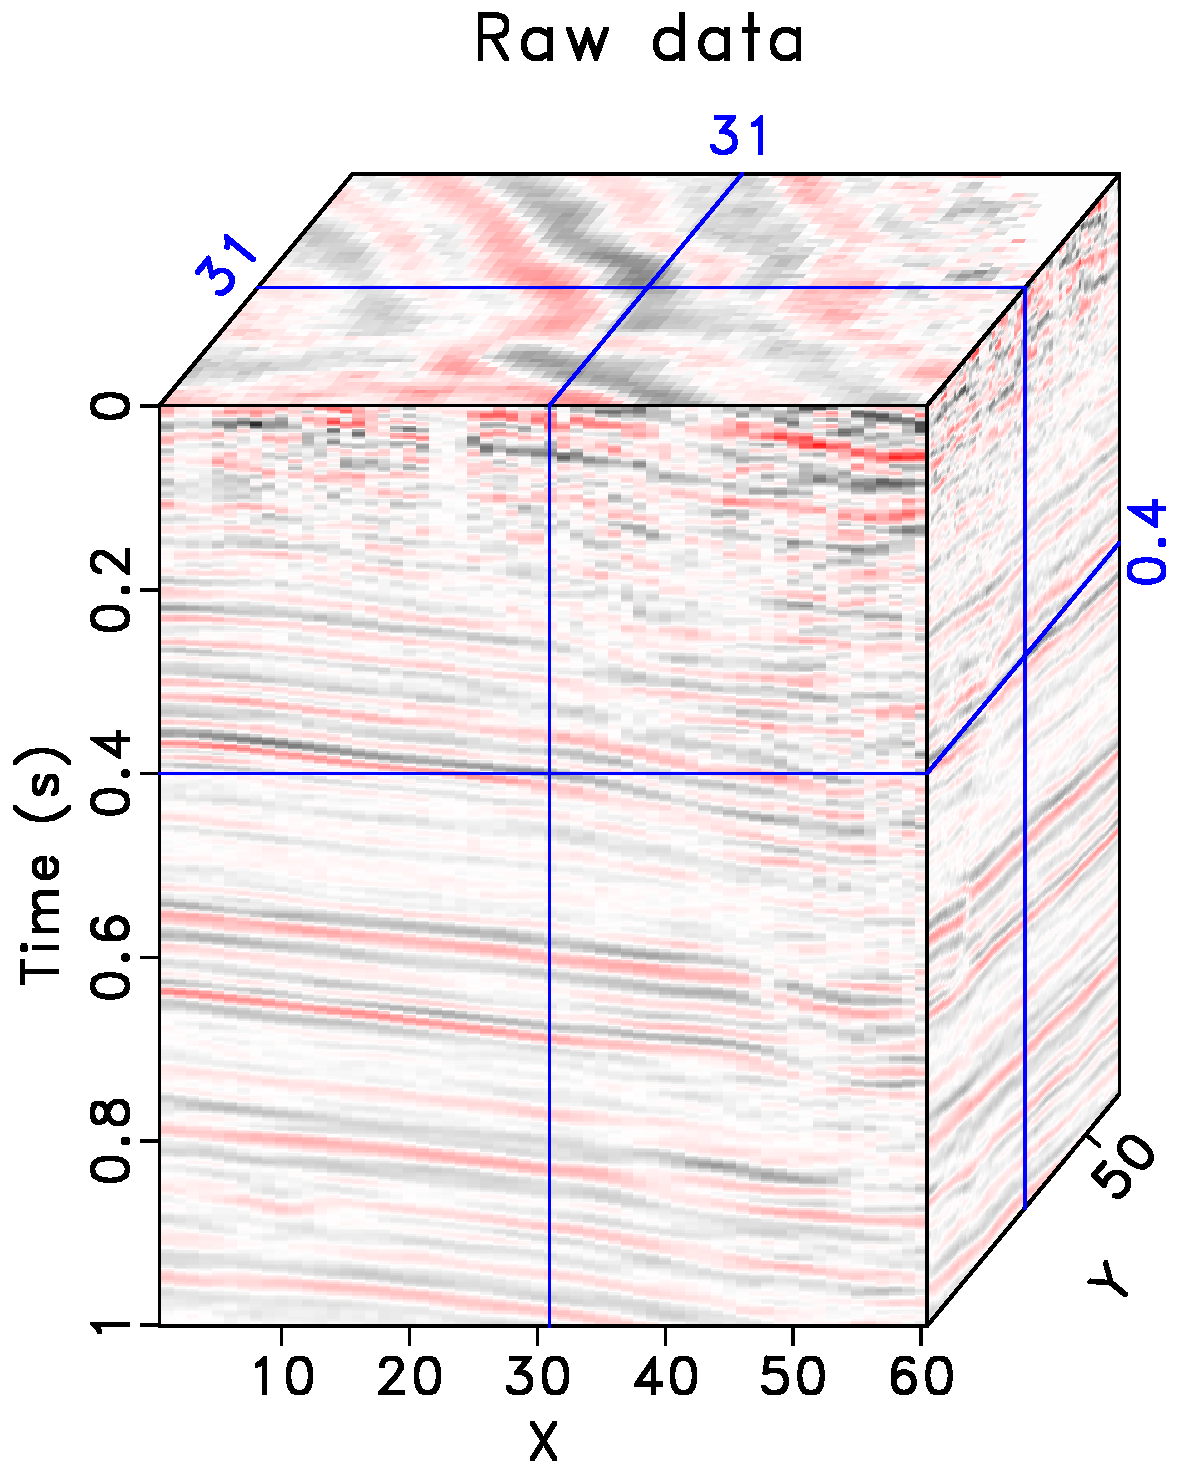
\includegraphics[width=0.23\textwidth]{Fig/real3}
   \label{fig:real3}}\\
 \subfloat[]{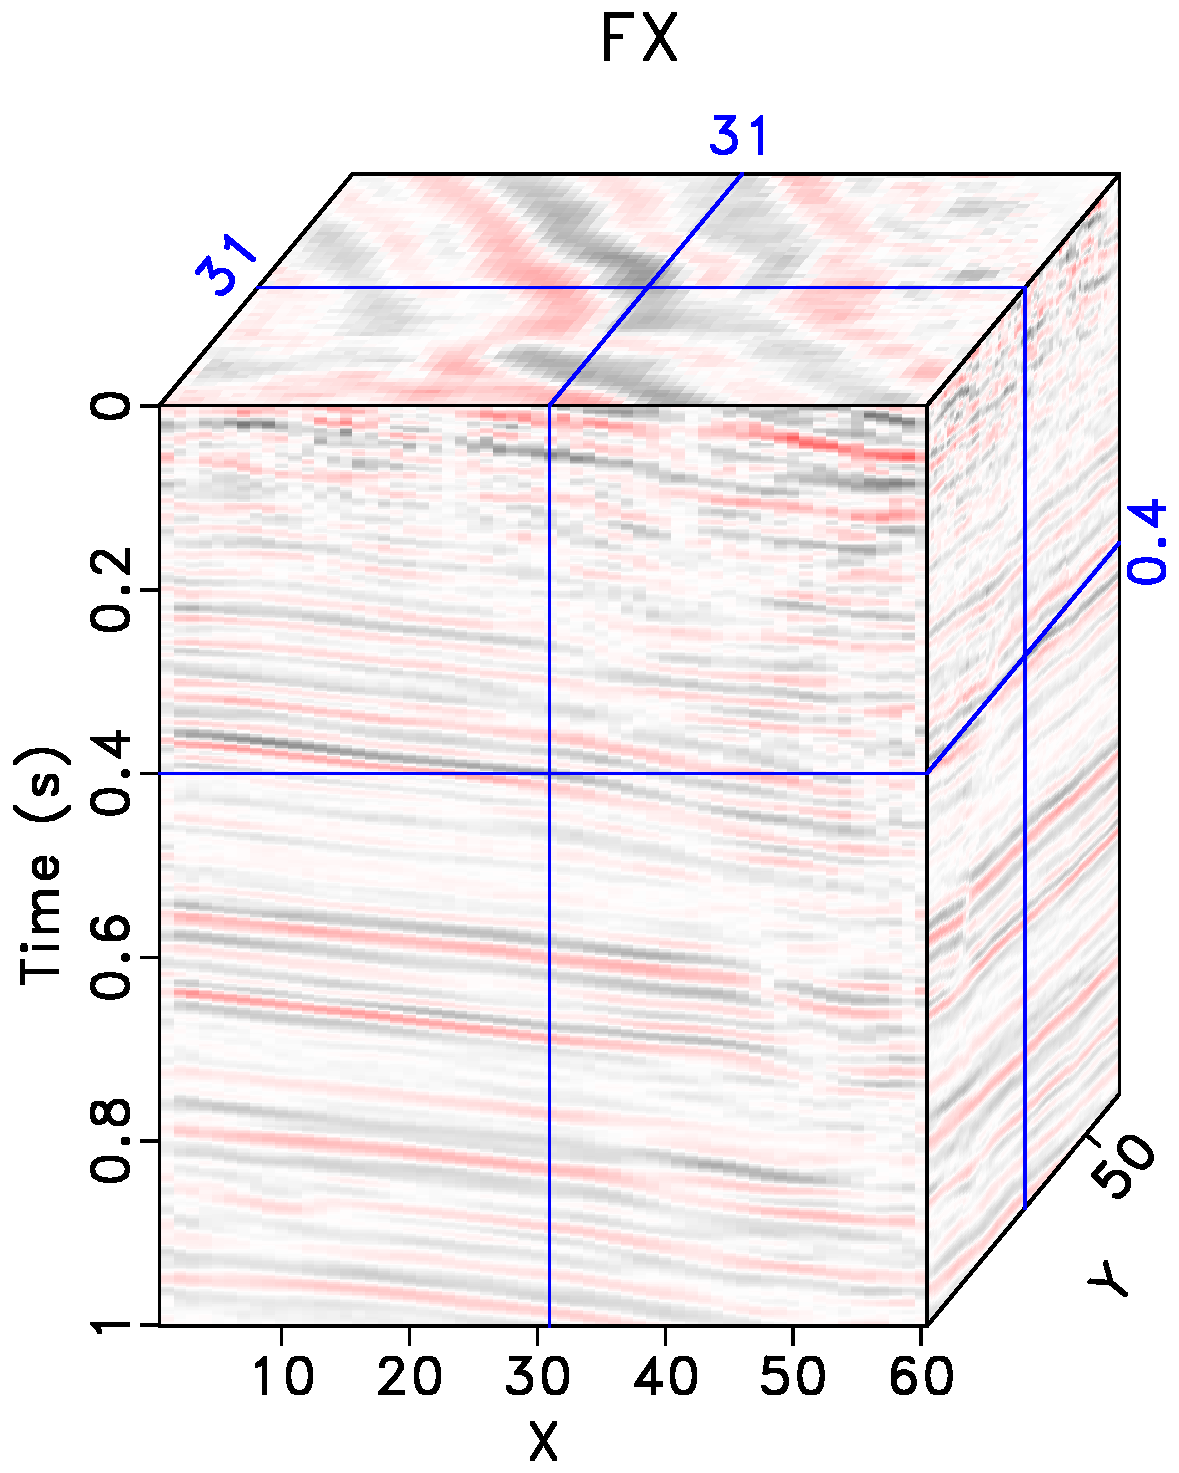
\includegraphics[width=0.23\textwidth]{Fig/real3-d2}
   \label{fig:real3-d2}}   
 \subfloat[]{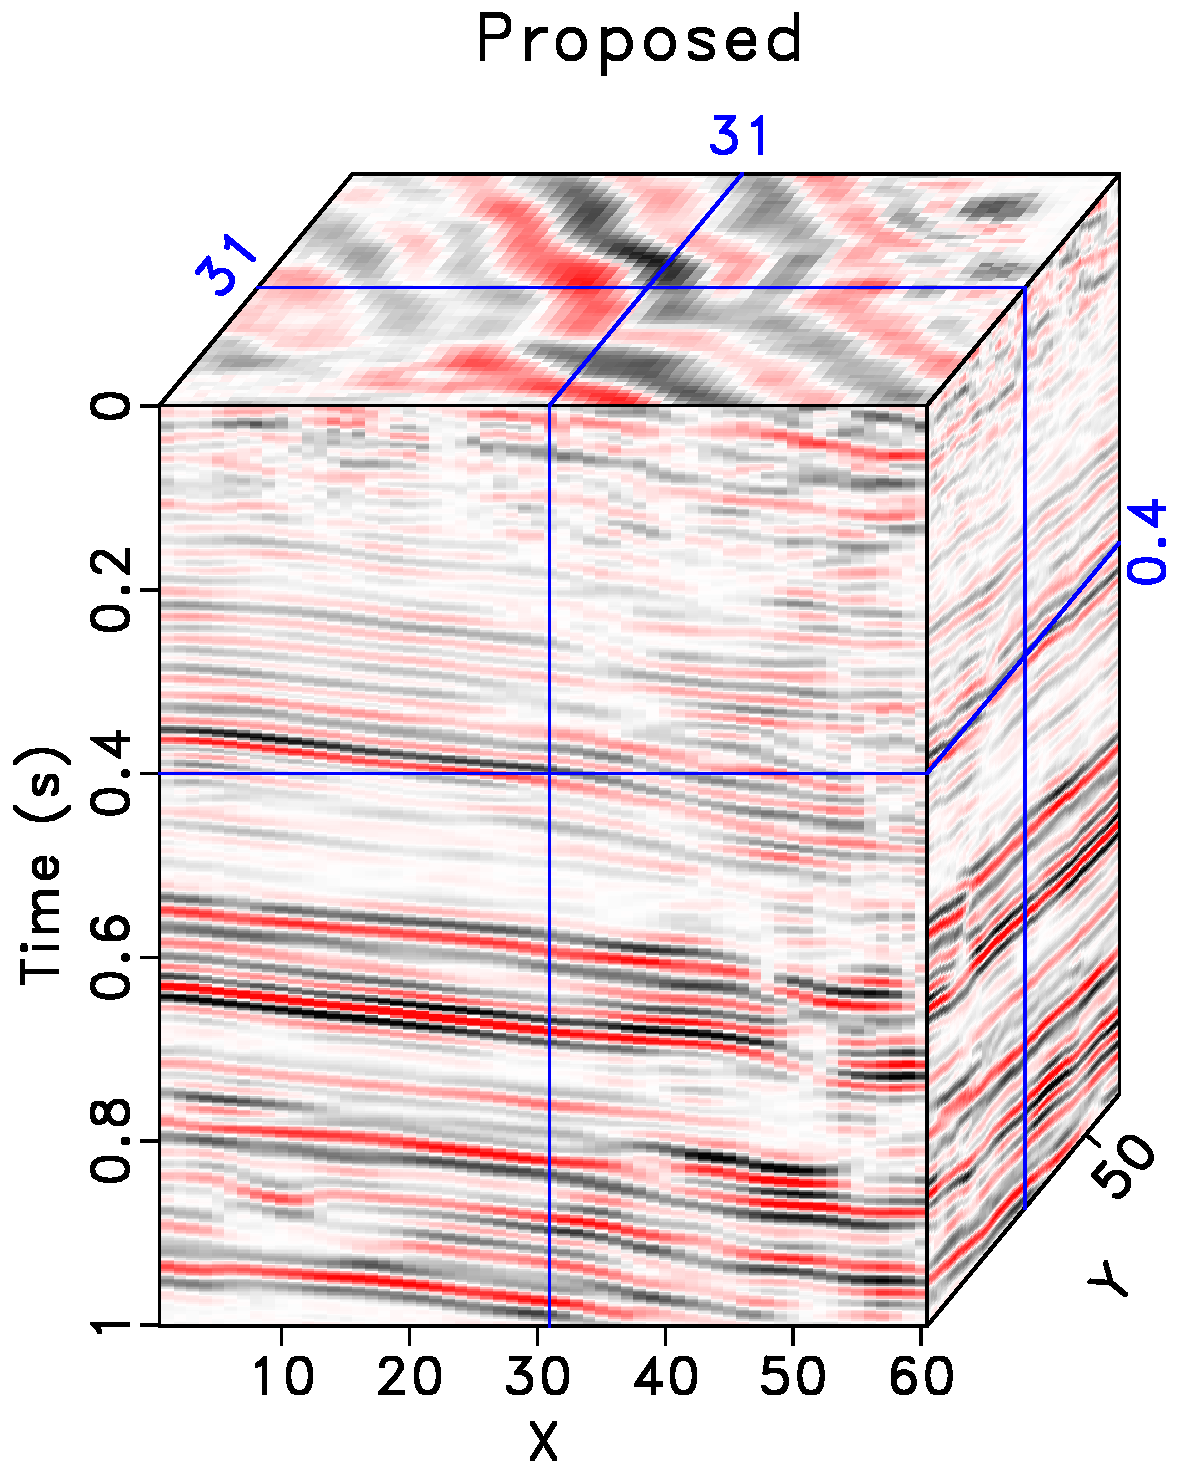
\includegraphics[width=0.23\textwidth]{Fig/real3-d1}
   \label{fig:real3-d1}}   
  \caption{3D seismic data example. (a) Raw data. (b) Denoised data using the FX method. (c) Q-compensated and denoised data using the proposed method.}
  \label{fig:real3,real3-d2,real3-d1}
\end{figure}

\begin{figure}[htb!]
 \centering
 \subfloat[]{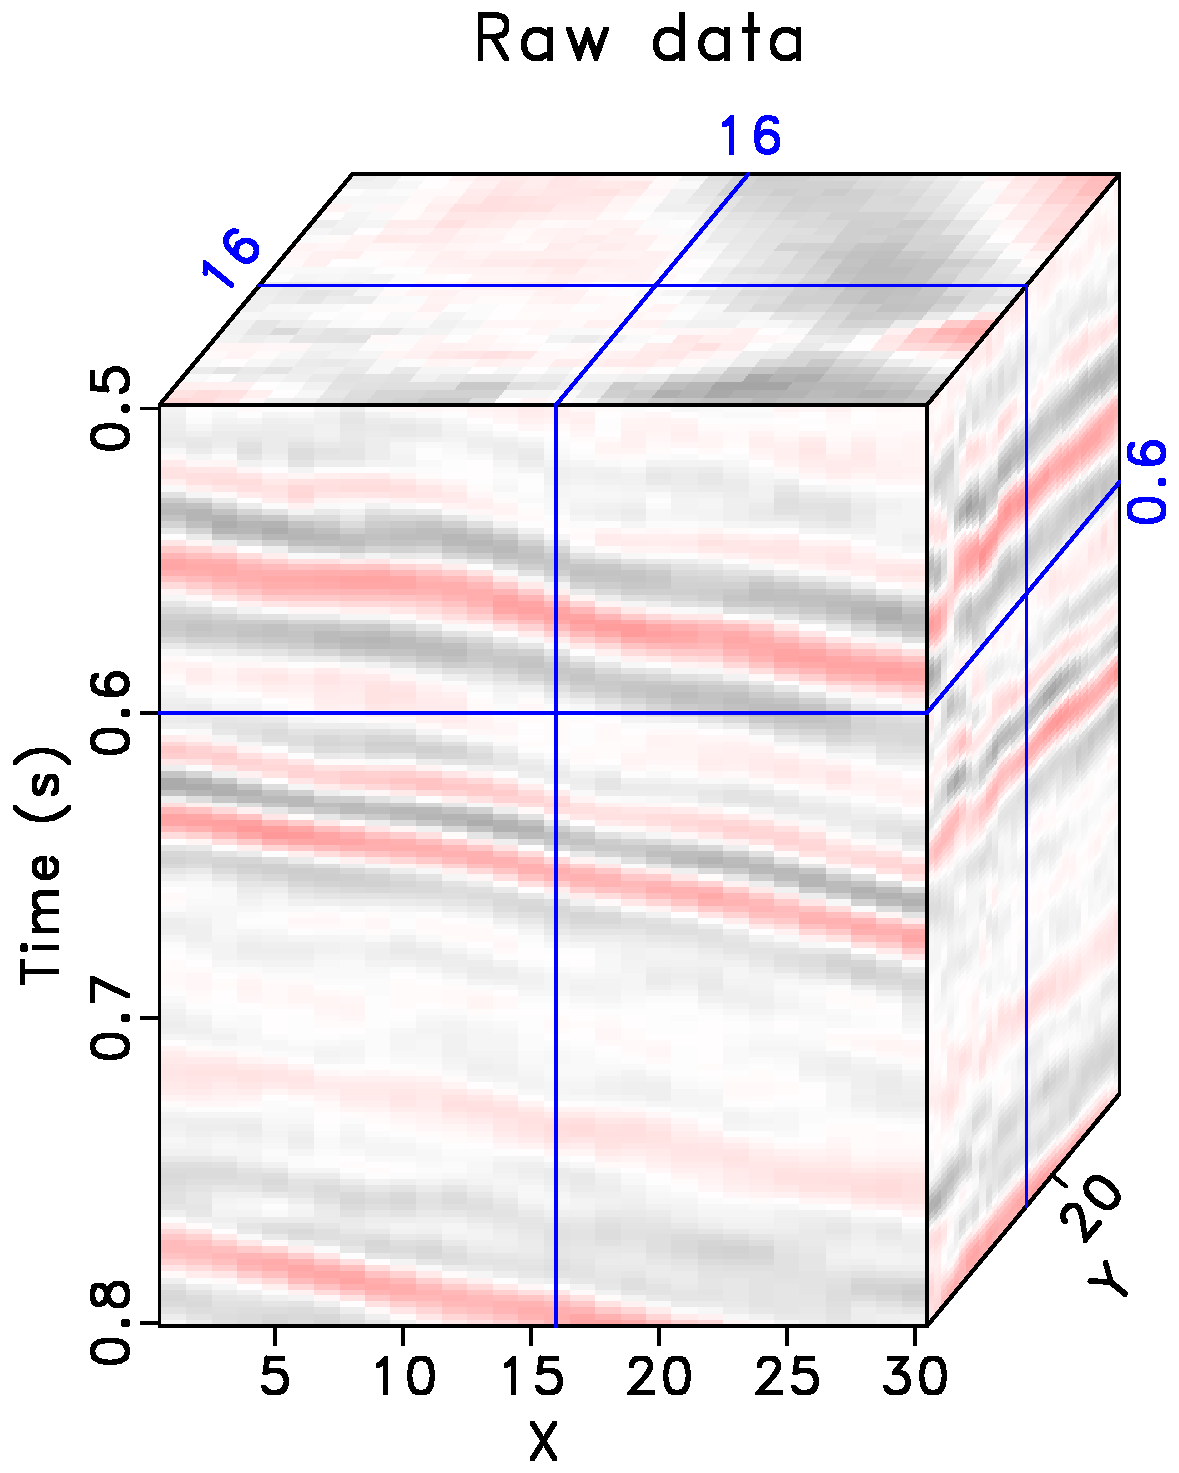
\includegraphics[width=0.23\textwidth]{Fig/real3-z}
   \label{fig:real3-z}}\\
 \subfloat[]{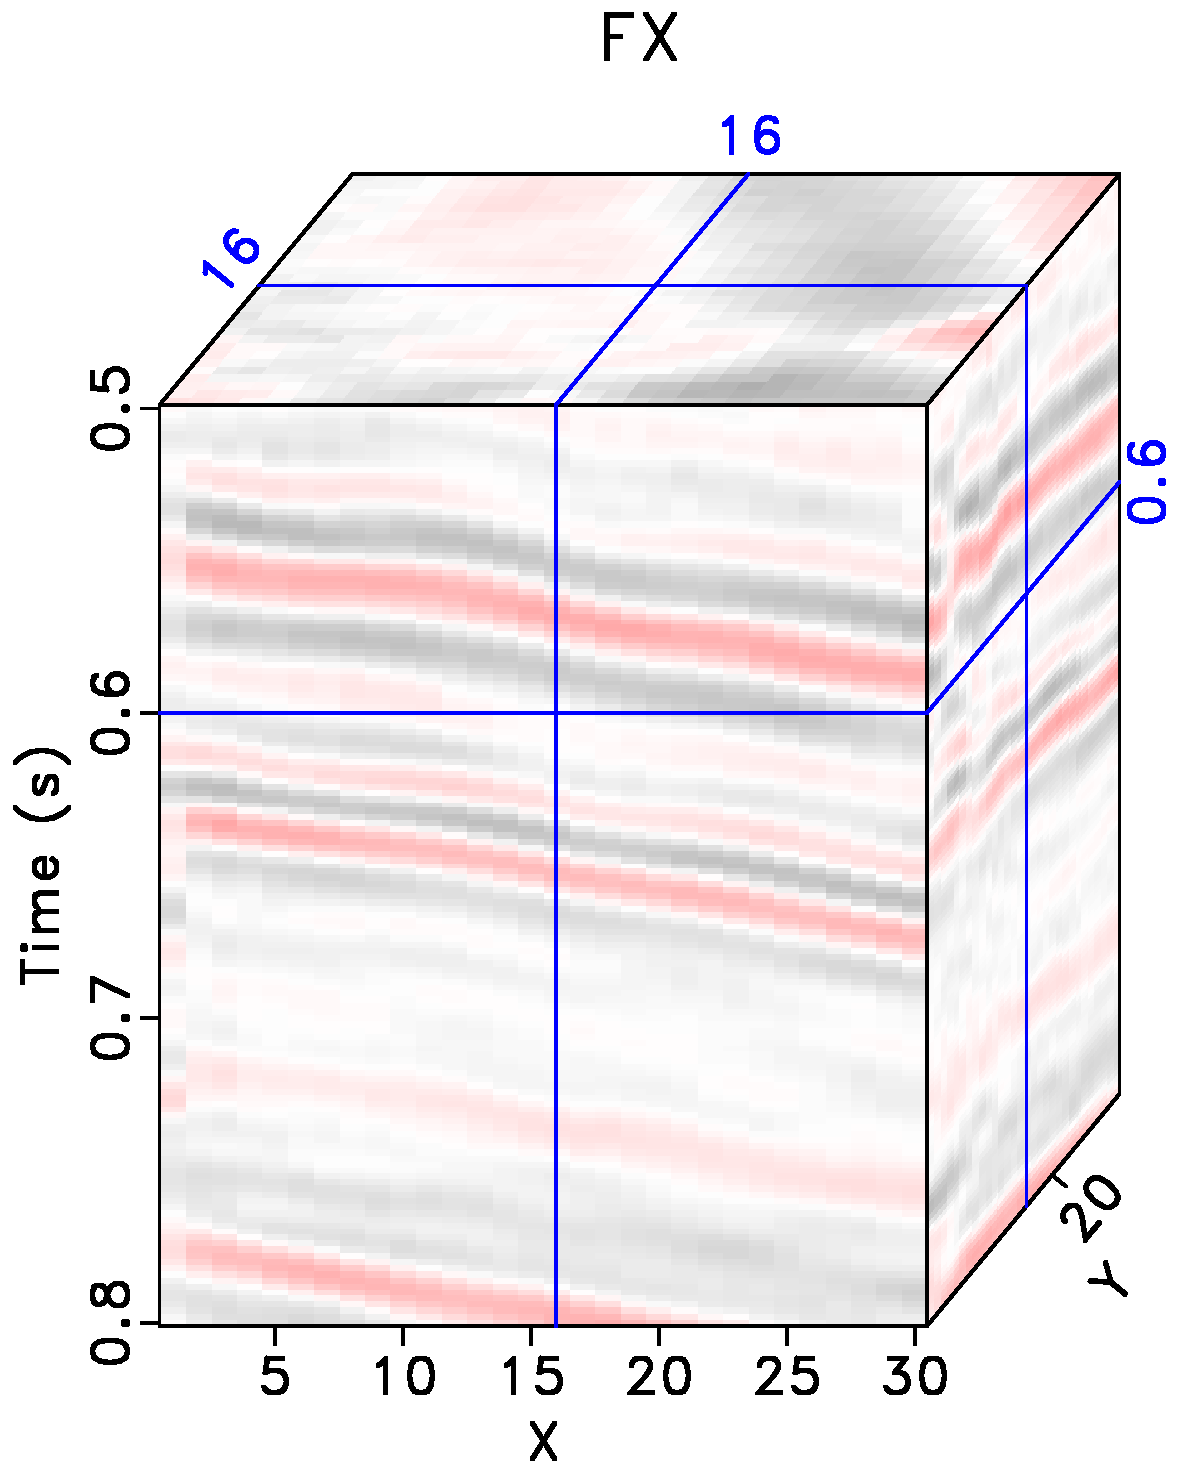
\includegraphics[width=0.23\textwidth]{Fig/real3-d2-z}
   \label{fig:real3-d2-z}}   
 \subfloat[]{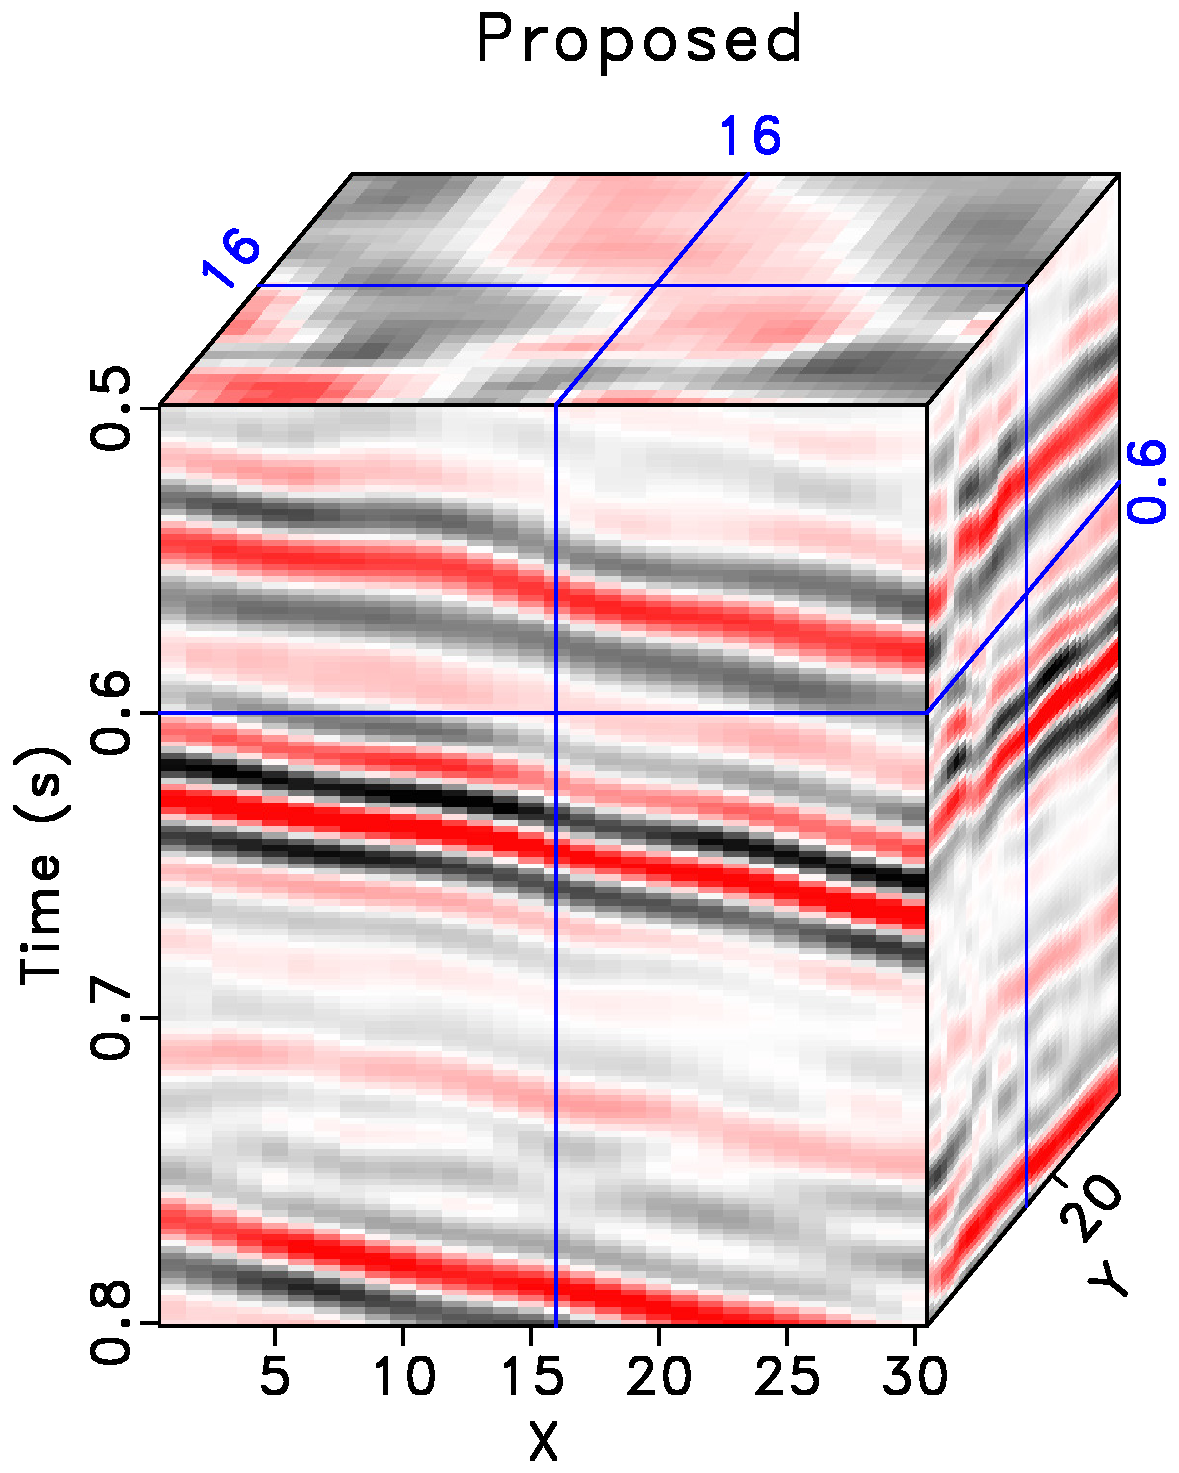
\includegraphics[width=0.23\textwidth]{Fig/real3-d1-z}
   \label{fig:real3-d1-z}}   
  \caption{Zoomed comparison of the 3D seismic data example. (a) Raw data. (b) Denoised data using the FX method. (c) Q-compensated and denoised data using the proposed method.}
  \label{fig:real3-z,real3-d2-z,real3-d1-z}
\end{figure}


\begin{figure}[htb!]
 \centering
 \subfloat[]{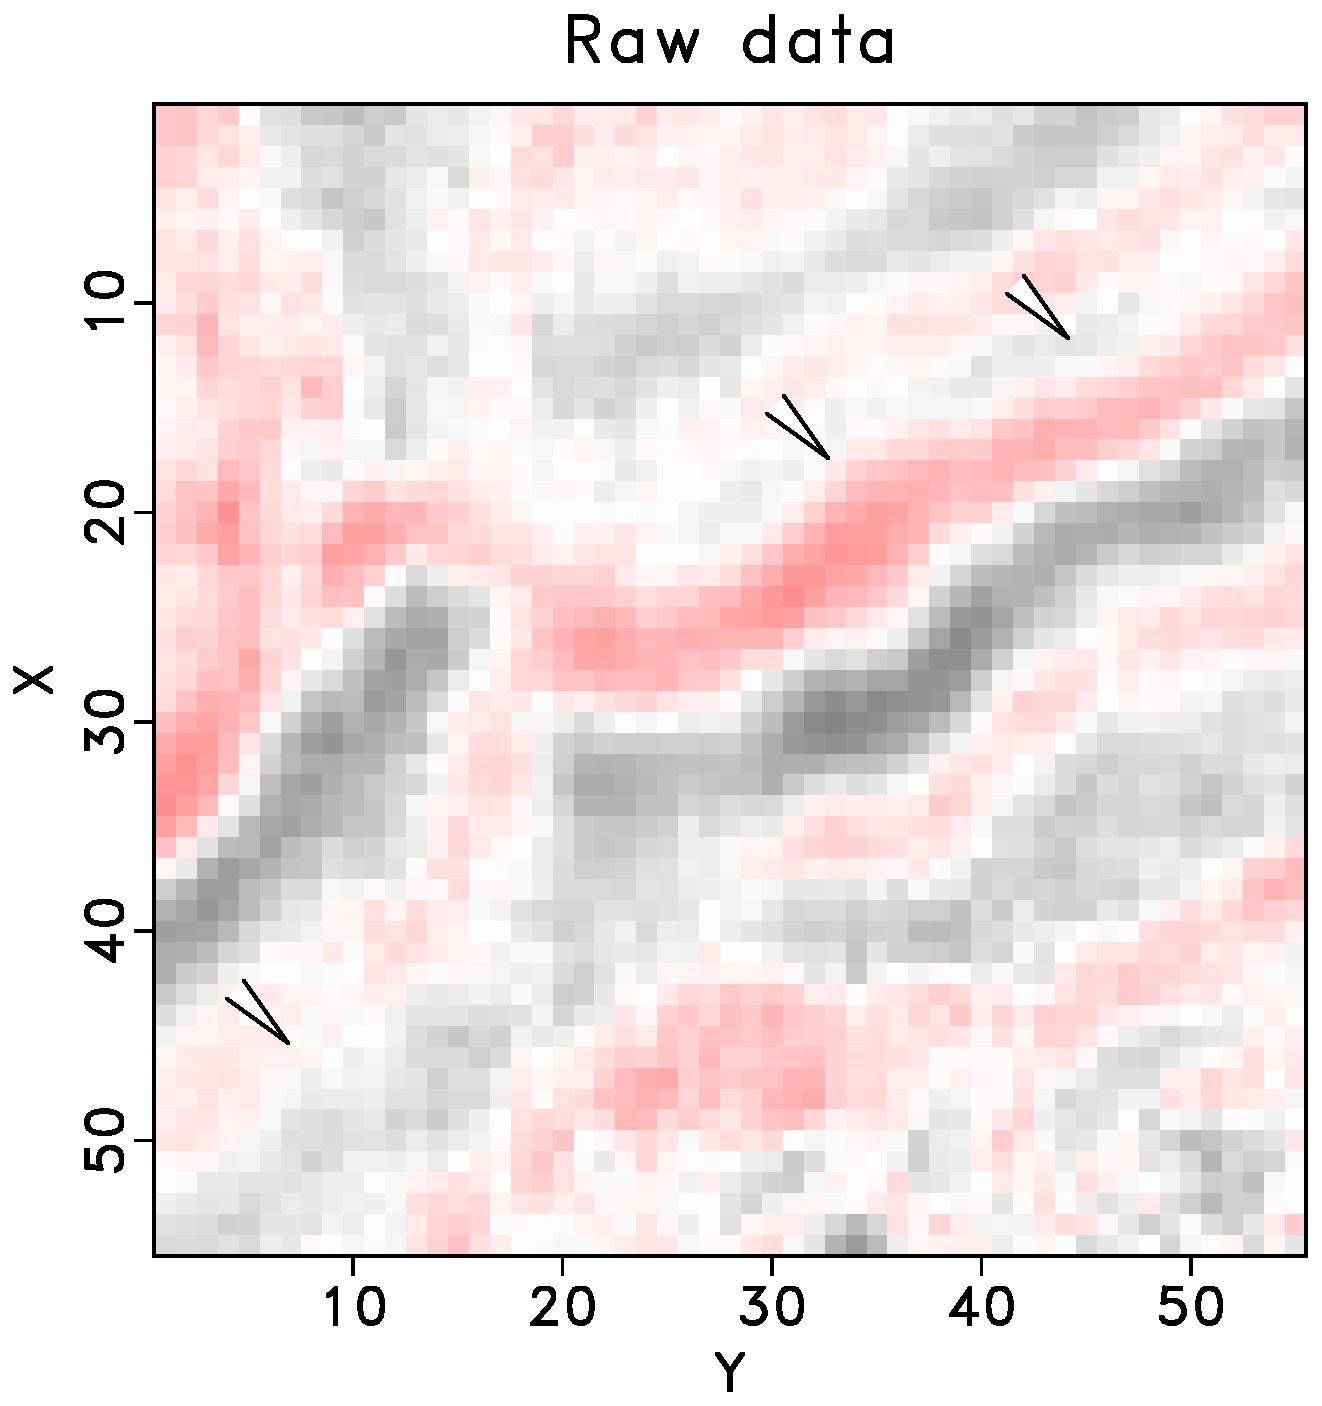
\includegraphics[width=0.33\textwidth]{Fig/real3-s-0}
   \label{fig:real3-s-0}}\\
 \subfloat[]{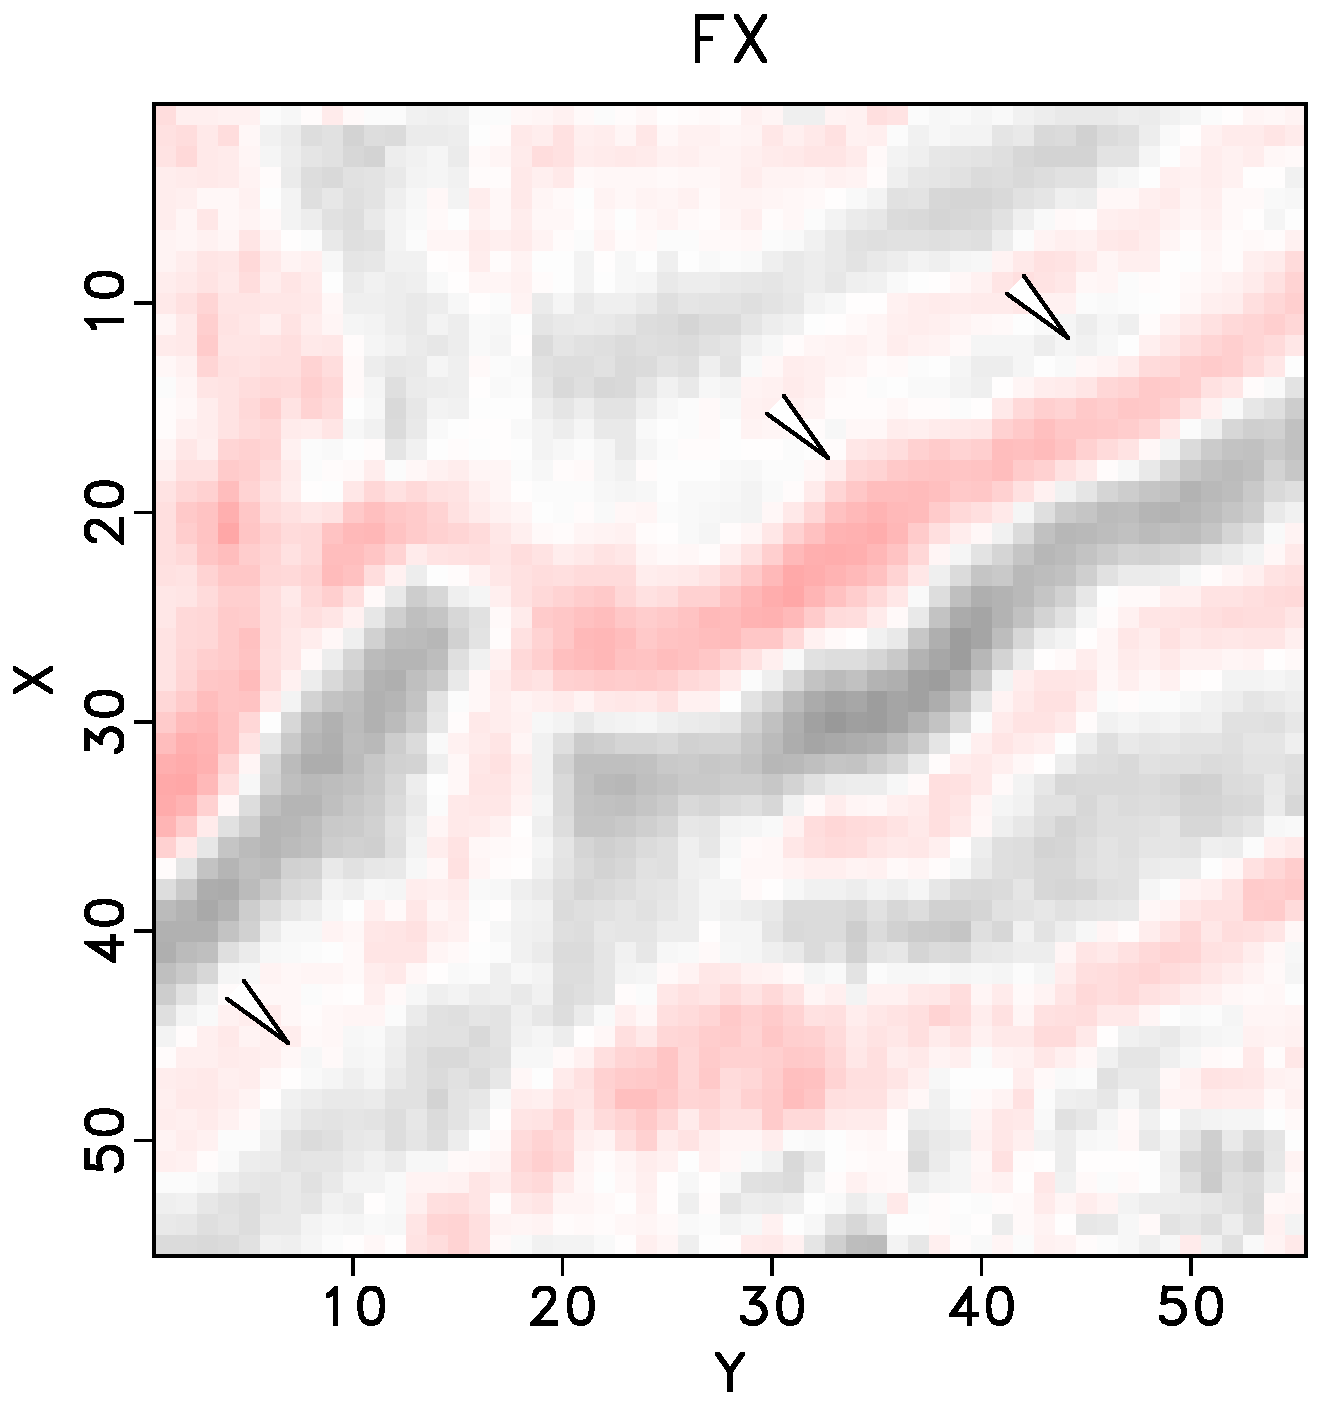
\includegraphics[width=0.33\textwidth]{Fig/real3-d2-s-0}
   \label{fig:real3-d2-s-0}} \\  
 \subfloat[]{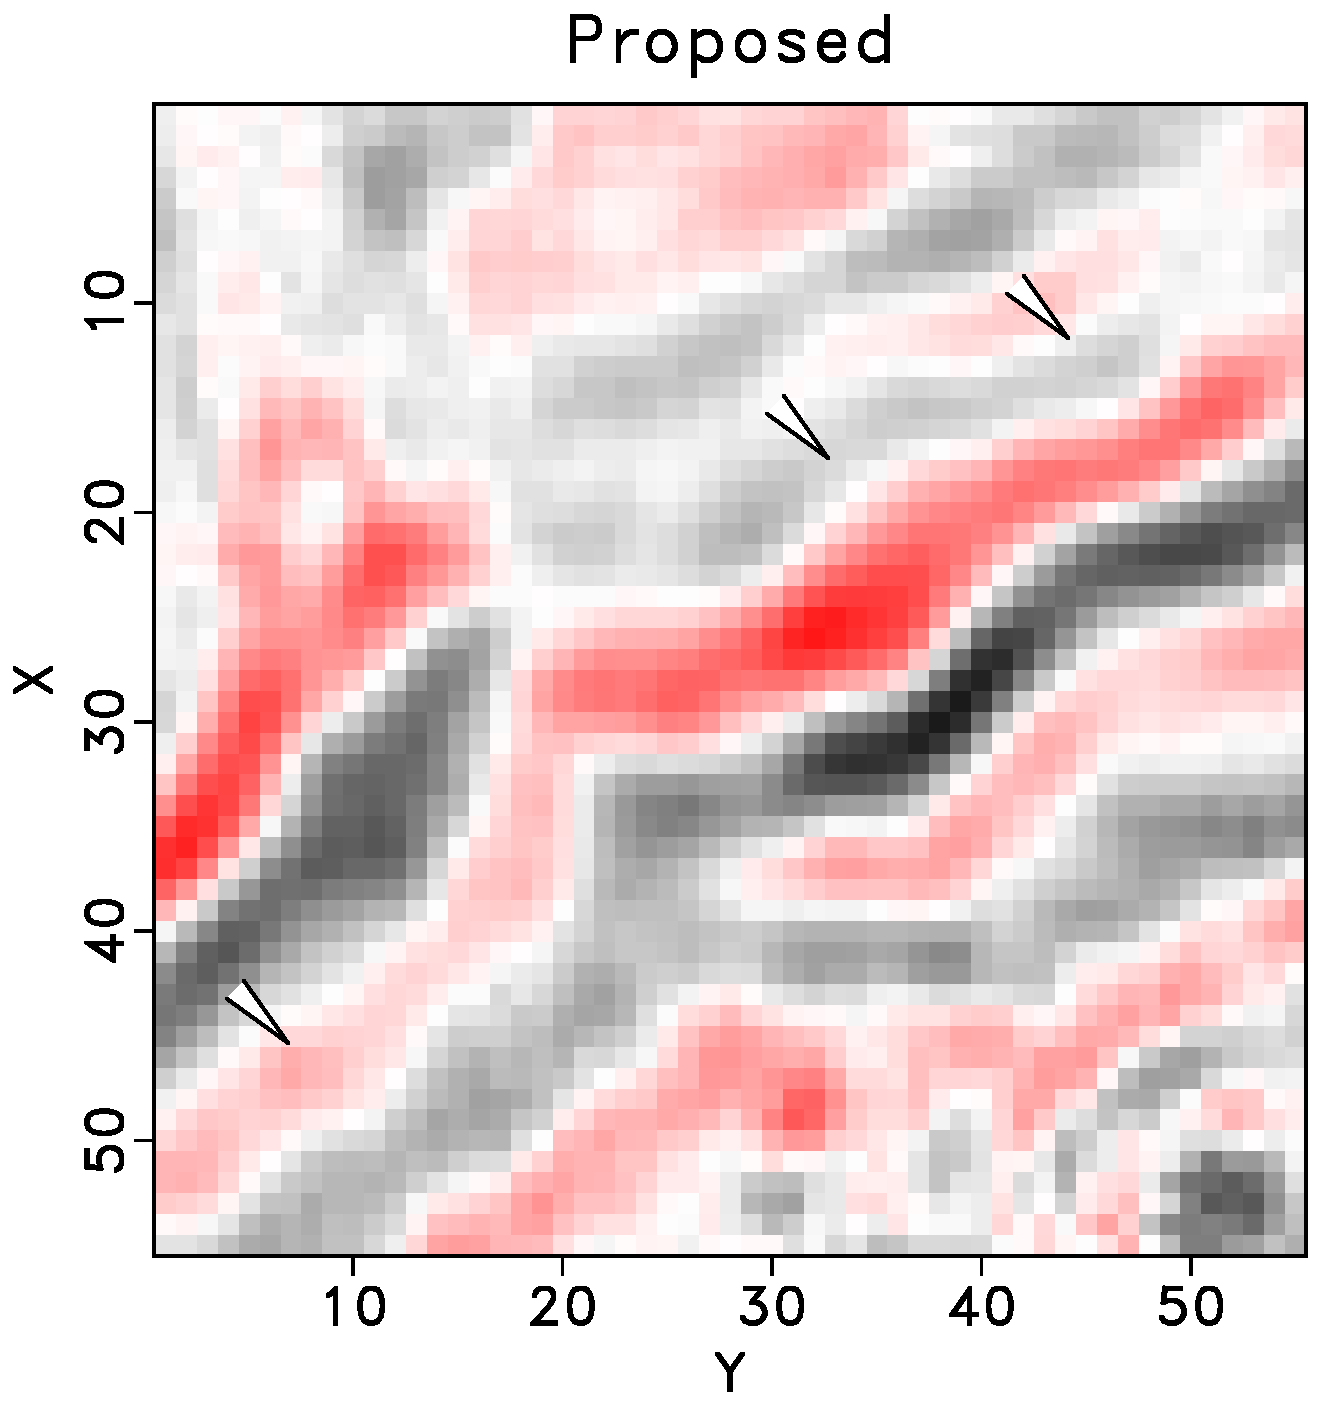
\includegraphics[width=0.33\textwidth]{Fig/real3-d1-s-0}
   \label{fig:real3-d1-s-0}}   
  \caption{Constant-time ($t=0.4s$) comparison of the 3D seismic data example. (a) Raw data. (b) Denoised data using the FX method. (c) Q-compensated and denoised data using the proposed method.}
  \label{fig:real3-s-0,real3-d2-s-0,real3-d1-s-0}
\end{figure}

\begin{figure}[htb!]
\centering
\subfloat[]{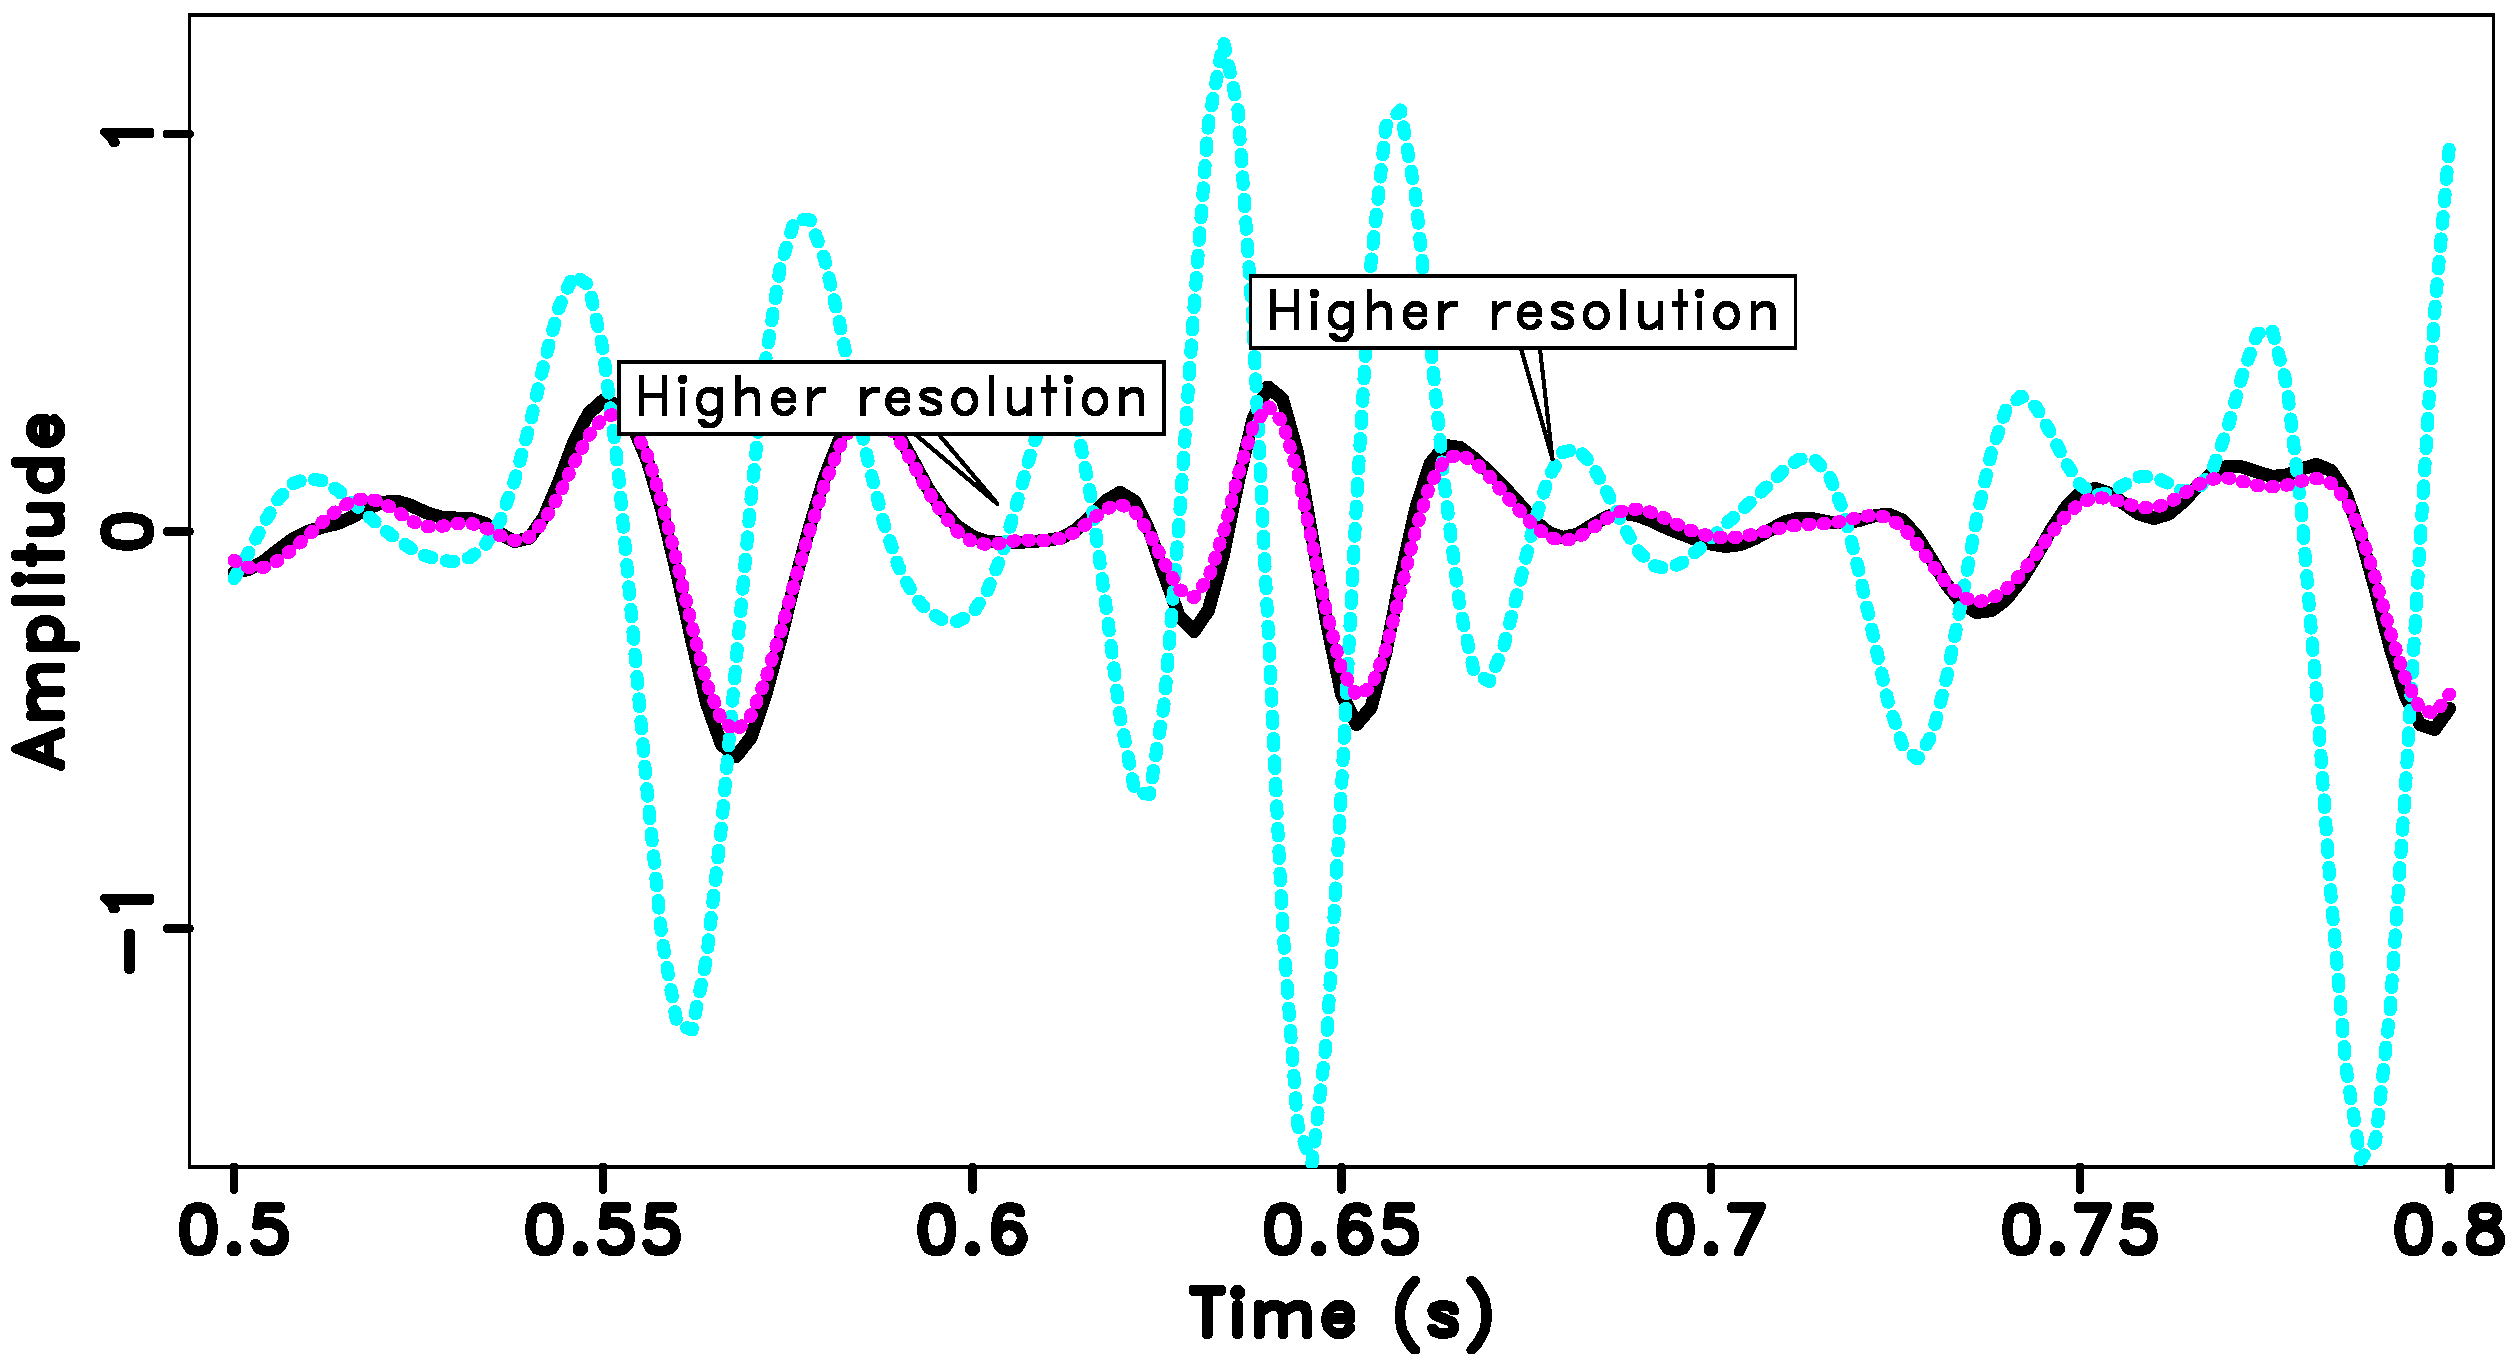
\includegraphics[width=0.5\textwidth]{Fig/real3-traces-0}}
\caption{\new{Trace-by-trace comparison (middle traces of the zoomed seismic cubes in Fig. \ref{fig:real3-z,real3-d2-z,real3-d1-z}). Black denotes the raw data. Pink denotes the FX method. Cyan denotes the proposed method. Note the obviously enhanced resolution.} }
\label{fig:real3-traces-0}
\end{figure}

\section{Examples}
We use several datasets to show the performance of the new Q-compensated denoising method, including a synthetic and two field data examples. First, the synthetic example is shown in Fig. \ref{fig:syn-dc}, which is a clean seismic section containing several linear events. Some of the events are crossing each other. We apply a forward attenuating operator ($\mathbf{A}$) introduced above with $Q=50$ to the clean seismic section, and show the attenuated data in Fig. \ref{fig:syn-da}. The wavelet we use here is a Ricker wavelet with 30 Hz dominant frequency. The deep seismic signals are of very weak amplitude due to the attenuation. We then add some band-limited random noise into the attenuated data and show the noisy and attenuated data in Fig. \ref{fig:syn-dn}. We apply the FX method \cite[]{canales1984} and the proposed signal enhancing method to the noisy and attenuated data, and then show the results in Fig. \ref{fig:syn-d2,syn-d1}. 

As can be seen from Fig. \ref{fig:syn-d2,syn-d1}, the FX method can suppress some random noise but cannot recover the amplitude loss. What is worse is that the FX method almost removes all the weak signals around 1.5s. The proposed method, however, can obtain an almost correct result with amplitude compensated and noise removed. The recovered seismic signals are very close to the ground-truth solution shown in Fig. \ref{fig:syn-dc}. To evaluate the denoising and Q-compensation performance, we use the local similarity metric \cite[]{fomel2007localattr,yangkang2015ortho}. We calculate the local similarity between the ground-truth solution (Fig. \ref{fig:syn-dc}) and all other data in Figs. \ref{fig:syn-dc,syn-da,syn-dn} and \ref{fig:syn-d2,syn-d1}. A higher local similarity value indicates a higher quality of the data to be evaluated since the signals are more similar to the ground-truth signals. The local similarity maps are plotted in Fig. \ref{fig:syn-da-simi,syn-dn-simi,syn-d2-simi,syn-d1-simi}. The local similarity comparison clearly shows that the proposed method obtains obviously higher local similarity values, and thus the proposed method obtains a very accurate recovery of the seismic signals. We then extract a single trace (the 3rd trace) from each seismic sections from Figs. \ref{fig:syn-dc,syn-da,syn-dn} and \ref{fig:syn-d2,syn-d1} and plot them in Fig. \ref{fig:syn-ss0,syn-ss-z}. Fig. \ref{fig:syn-ss0} plots the trace-by-trace comparison in the original scale, where the ground-truth solution is denoted by the black line. The red line denotes the clean attenuated data. The pink line corresponds to the noisy attenuated data.  The green line corresponds to the proposed Q-compensated denoising method. The blue line corresponds to the FX method. It is clear that the black and green lines are almost overlapping, indicating an excellent amplitude recovery performance. We zoom a waveform and show the comparison in Fig. \ref{fig:syn-ss-z}. The zooming part is stressed by the cyan frame box in Fig. \ref{fig:syn-ss0}. 

The first field data example is a 2D section, as shown in Fig. \ref{fig:real-dn-0}. The seismic data contains several representative features, e.g., many fault structures in the shallow area and some highly dipping structures in the deep area probably caused by abrupt uplifting of deep stratas. However, due to \new{the} strong random noise and existence of the wave attenuation phenomenon, the seismic events are highly discontinuous, affecting the interpretation challenges in this geological area.  Traditionally, we apply a denoising operator to the raw seismic data and obtain an improved seismic section. For example, we can apply the FX method to the raw data and obtain the denoised data shown in Fig. \ref{fig:real-d2-0}. The seismic events become more continuous but still have some sporadic weak-amplitude patterns which are caused by the strong wave attenuation. We apply the proposed Q-compensated denoising method to the raw data and obtain a much improved section, as shown in Fig. \ref{fig:real-d1-0}. It is clear that the amplitude loss is recovered well and the signal-to-noise ratio is increased dramatically. In this field data test, we assume a constant $Q=50$ for the convenient processing. For a better comparison, we zoomed two parts from each sub-figure in Fig. \ref{fig:real-dn-0,real-d2-0,real-d1-0}.  The zooming sections highlighted by the pink frame box are plotted in Fig. \ref{fig:real-dn-z1,real-d2-z1,real-d1-z1}. It becomes very clear that the proposed approach can obtain a good amplitude recovery and denoising. The seismic events become obviously continuous and the fault structures become very clearly depicted. Because of the Q-compensation, the resolution of the processed data is also dramatically enhanced, which is beneficial to interpret the thin-bed structures. Another area that is stressed using the red rectangles in Fig. \ref{fig:real-dn-0,real-d2-0,real-d1-0} is zoomed and compared in Fig. \ref{fig:real-dn-z2,real-d2-z2,real-d1-z2}. It is more obvious that some thin layers that have \new{a} very weak amplitude in the raw seismic data have been revealed clearly after the Q-compensated and denoising processing, e.g., in areas around 2.4 sec and between 200th and 250th traces. To evaluate the influence of different Q values to the result, we use six different Qs, i.e., Q=60, 70, 80, 90, 100, and 120, to process the data based on the same aforementioned framework, and show the results in Fig. \ref{fig:real-d1-q60-0,real-d1-q70-0,real-d1-q80-0,real-d1-q90-0,real-d1-q100-0,real-d1-q120-0}. For a better view, we zoom the area pointed out by the pink frame boxes and show the comparison in Fig. \ref{fig:real-d1-q60-z1,real-d1-q70-z1,real-d1-q80-z1,real-d1-q90-z1,real-d1-q100-z1,real-d1-q120-z1}. It is obvious that as Q increases, the amplitude compensation effect becomes weaker, and the seismic events become less continuous. It is easy to infer that as Q becomes very large, there is little effect on improving the quality of the seismic data. According to our experience, when Q becomes very small, e.g., less than 40, the proposed method is more likely to cause instability due to much boosted noise energy.  In practice, we are recommending starting tuning the proposed algorithm with Q=50, and then gradually increase the Q value to see which result best serves the geological interpretation.  

Finally, we use a 3D seismic dataset to demonstrate the proposed method. Fig. \ref{fig:real3} demonstrates the raw seismic data. Fig. \ref{fig:real3-d2} shows the result from \old{a}\new{the} FX method. For simplicity, we only use the 2D version of the predictive filtering method to denoise this data, i.e., process the data in a 2D section. Although the simple denoising method can attenuate some random noise, it cannot compensate for the amplitude loss due to seismic attenuation. The amplitude of the deep area is still weak. We apply the proposed Q-compensated denoising method to the raw data and show the result in Fig. \ref{fig:real3-d1}. The amplitude of the deep areas \old{have}\new{has} been enhanced significantly. We zoomed a 3D cube from each dataset in the original scale and show the comparison in Fig. \ref{fig:real3-z,real3-d2-z,real3-d1-z}, where we can better see that the proposed method not only suppress random noise, but also compensate for the amplitude loss and enhance the vertical resolution.  We also extract a constant-time slice of $t=0.4$s from each dataset in Fig. \ref{fig:real3,real3-d2,real3-d1} and show the comparison in Fig. \ref{fig:real3-s-0,real3-d2-s-0,real3-d1-s-0}. It is clear that the proposed method \old{unveil}\new{unveils} several hidden signals from the raw data thanks to the Q compensation, as indicated by the arrows \new{in Fig. \ref{fig:real3-d1-s-0}}.  \new{A trace-by-trace comparison is plotted in Fig. \ref{fig:real3-traces-0}, where the black line denotes the raw data. The pink line corresponds to the result from the FX method. The cyan line corresponds to the proposed method. It is clear that the proposed method significantly enhance the resolution. }




%\section{Discussions}
\section{Conclusions}
Both seismic noise and seismic attenuation can cause the low-quality issue of many reflection seismic data. We have introduced an inversion framework to simultaneously remove seismic noise and compensate for the amplitude absorption and phase distortion, thereby enhancing the resolution and signal-to-noise ratio (SNR) of the seismic data. We theoretically introduce the forward operator in the inverse problem, and use the L1-norm constrained optimization problem to solve the inverse problem. A preconditioned conjugate gradient method is used to solve the optimization problem with superb performance. \new{Due to the inversion process, the computational cost of the proposed method is higher than a traditional denoising algorithm. However, the computational complexity can be controlled by the numbers of inner and outer iterations, i.e., $N_i$ and $N_o$. Since the attenuation compensation could boost the high-frequency energy, thus it could be more sensitive to the noise levels than a standard denoising algorithm.} All synthetic, 2D and 3D real post-stack seismic data containing strong random noise are tested with the proposed method to demonstrate its validity in industrial applications.


%\inputdir{synth}
%%\plot{test1}{width=\textwidth}{Separated x-component of the S1 elastic wavefield in the orthorhombic media.}
%\multiplot{3}{syn-dc,syn-da,syn-dn}{width=0.4\textwidth}{Synthetic data example. (a) Clean data. (b) Noisy data with attenuated amplitude. (c) Enhanced data using fx method. (d) Enhanced data using the proposed method.}
%






\bibliographystyle{seg}
\bibliography{q}

